\section{Auswertung}
\label{sec:Auswertung}
Jegliche Fehlerrechnung wurde mit der Python-Bibliothek uncertainties \cite{uncertainties} absolviert. Trotz dessen sind die Formeln für
die Unsicherheiten in den jeweiligen Abschnitten angegeben.  Allgemeine Rechnungen wurden mit der Python-Bilbiothek numpy \cite{numpy} automatisiert.
\subsection{Wheatstonesche Brücke}
\label{sec:Wheat}
Mit der Wheatstoneschen Brückenschaltung sollten zwei Unbekannte Widerstände ermittelt werden.
In der folgenden Tabelle werden die Messwerte $R_2$ und $\sfrac{R_3}{R_4}$ der Messreihe aufgelistet. Zudem ist der mit Hilfe von Gleichung $\ref{eqn:wheat}$ berechnete 
Wert für $R_\text{x}$ eingetragen. Der Fehler lässt sich mit Hilfe der Gaußschen Fehlerfortpflanzung
\begin{equation}
  \label{eqn:fehR}
  \symup{\Delta}R_x=\sqrt{\left(\frac{R_3}{R_4}\right)^2  \left(\symup{\Delta}R_2\right)^2 + R_2^2  \left(\symup{\Delta}\frac{R_3}{R_4}\right)^2}
\end{equation}
berechnen. Die Fehler sind durch $\symup{\Delta}R_2$ = $\pm \, \num{0.002} \, R_2$
und $\symup{\Delta}\frac{R_3}{R_4}$ = $\pm \,  \num{0.005} \, \frac{R_3}{R_4}$ gegeben.
\begin{table}
  \centering
  \caption{Messwerte und berechnete Werte für Widerstand $R_\text{x}$ (Wert 10)}
  \label{tab:Wheat}
  \sisetup{table-format = 4}
  \begin{tabular}{
    c
    S[table-format = 4.2] @{${}\pm{}$} S[table-format=1.2]
    S[table-format=1.2] @{${}\pm{}$} S[table-format=1.2]
    S[table-format = 3.2] @{${}\pm{}$} S[table-format=1.2]}
     \toprule
     {Wert 10}  &
     \multicolumn{2}{c}{$R_2 \mathbin{/} \si{\ohm}$}       &
     \multicolumn{2}{c}{$\frac{R_3}{R_4}$}       & 
     \multicolumn{2}{c} {$R_\text{x}  \mathbin{/} \si{\ohm}$}\\
     \cmidrule(lr){2-3} \cmidrule(lr){4-5} \cmidrule(lr){6-7}
     \midrule
     Messung 1 & 332.00  & 0.66 & 0.72 & 0.00 & 240.41 & 1.30\\
     Messung 2 & 664.00  & 1.33 & 0.36 & 0.00 & 238.17 & 1.28\\
     Messung 3 & 1000    & 2    & 0.24 & 0.00 & 239.93 & 1.29\\
      \bottomrule
  \end{tabular}
\end{table}%
Der Mittelwert von $R_\text{x}$ lässt sich mit   
\begin{equation}
  \label{eqn:mit}
  \bar{R}_\text{x}=\sum_{i=1}^3 \frac{1}{3}R_{x_i}
\end{equation}
berechnen. Daraus folgt für den Mittelwert des Widerstands Wert 10 $\bar{R}_\text{x}= \SI{239.5(7)}{\ohm}$.
Äquivalent dazu wurden auch die Werte von dem anderen unbekannten Widerstand ermittelt und eingetragen.
\begin{table}
  \centering
  \caption{Messwerte und berechnete Werte für Widerstand, $R_\text{x}$ (Wert 11)}
  \label{tab:Wheatr}
  \sisetup{table-format = 4.2}
  \begin{tabular}{
    c
    S @{${}\pm{}$} S[table-format=1.2]
    S[table-format=1.2] @{${}\pm{}$} S[table-format=1.2]
    S[table-format = 3.2] @{${}\pm{}$} S[table-format=1.2]}
     \toprule
     {Wert 11}  &
     \multicolumn{2}{c}{$R_2 \mathbin{/} \si{\ohm}$}       &
     \multicolumn{2}{c}{$\frac{R_3}{R_4}$}       & 
     \multicolumn{2}{c} {$R_\text{x}  \mathbin{/} \si{\ohm}$}\\
     \cmidrule(lr){2-3} \cmidrule(lr){4-5} \cmidrule(lr){6-7}
     \midrule
     Messung 1 &  332.00  & 0.66  & 1.48 & 0.01 & 491.82 & 2.65\\
     Messung 2 &  664.00  & 1.33  & 0.74 & 0.00 & 488.78 & 2.63\\
     Messung 3 & 1000     & 2     & 0.49 & 0.00 & 492.54 & 2.65\\
      \bottomrule
  \end{tabular}
\end{table}
Mit der Formel für den Mittelwert \eqref{eqn:mit} folgt für Wert 11 $\bar{R}_\text{x}=\SI{491\pm1.5}{\ohm}$.
\subsection{Kapazitätsmessbrücke}
\label{subsec:kapaaus}
Hierbei ist der Kondensator durch einen ohmschen Widerstand und eine widerstandslose Kapazität ersetzt worden.
Zur Brechnung der Werte wurde die Gleichung $\ref{eqn:capmes}$ genutzt.
Alle Messwerte, berechneten Kapazitäten und Widerstände für den Wert 8 sind in der Tabelle \ref{tab:kapa} aufgeführt.
Dabei wurden die Fehler des Widerstands mit der Formel \eqref{eqn:fehR} und
die der Kapazität mit
\begin{equation}
  \symup{\Delta}C_x=\sqrt{\left(\frac{R4}{R3}\right)^2 \cdot \left(\symup{\Delta}C_2\right)^2
  +\left(-C_2\frac{R4}{R3}\right)^2 \cdot \left(\symup{\Delta}\frac{R4}{R3}\right)^2}
\end{equation}
berechnet. Wobei $\symup{\Delta}R_2=\pm \, \num{0.03} \, R_2$ der Fehler von dem variablen Widerstand ist und $\symup{\Delta}C_2=\pm \, \num{0.002} \, C_2$ der Fehler 
der Kapazität. Die Abweichung von $\frac{R_3}{R_4}$ ist dieselbe Abweichung wie in Abschnitt \ref{sec:Wheat}.
\begin{table}
  \centering
  \caption{Messwerte und berechnete Werte für realen Kondensator,
  $R_\text{x}$ und $C_\text{x}$ \\(Wert 8)}
  \label{tab:kapa}
  \sisetup{table-format = 3}
  \begin{tabular}{
    c
    S[table-format = 3.2] @{${}\pm{}$} S[table-format=2.2]
    S[table-format = 1.2] @{${}\pm{}$} S[table-format=1.2]
    S[table-format = 3.2] @{${}\pm{}$} S[table-format=1.2]
    S[table-format = 3.2] @{${}\pm{}$} S[table-format=2.2]
    S[table-format = 3.2] @{${}\pm{}$} S[table-format=1.2]}
     \toprule
     {Wert 8}  &
     \multicolumn{2}{c}{$R_2 \mathbin{/} \si{\ohm}$}       &
     \multicolumn{2}{c}{$\frac{R_3}{R_4}$}                 & 
     \multicolumn{2}{c}{$C_2 \mathbin{/} \si{\nano\farad}$} &
     \multicolumn{2}{c}{$R_\text{x} \mathbin{/} \si{\ohm}$}&
     \multicolumn{2}{c} {$C_\text{x}  \mathbin{/} \si{\nano\farad}$}\\
     \cmidrule(lr){2-3} \cmidrule(lr){4-5} \cmidrule(lr){6-7} \cmidrule(lr){8-9} \cmidrule(lr){10-11}
     \midrule 
     Messung 1 & 371.00  & 11.13  & 1.54 & 0.01 & 450.0  & 0.9  & 570.62& 17.35 & 292.57 & 1.58\\
     Messung 2 & 418.00  & 12.54  & 1.37 & 0.01 & 399.00 & 0.79 & 572.52& 17.41 & 291.31 & 1.57\\
     Messung 3 & 278.00  &  8.34  & 2.06 & 0.01 & 597.00 & 1.19 & 572.15& 17.40 & 290.07 & 1.56\\
      \bottomrule
  \end{tabular}
\end{table}
Der Mittelwert für $R_\text{x}$ und $C_\text{x}$ wird ermittelt mit Gleichung \ref{eqn:mit} und mit
\begin{equation}
  \label{eqn:mit2}
  \bar{C_\text{x}}=\sum_{i=1}^3 \frac{1}{3}C_{x_i}\, .
\end{equation}
Somit ergibt sich für den Kondensator mit Wert 8 eine Kapazität von $\bar{C}_\text{x}=\SI{291.3 \pm 0.9}{\nano\farad}$ und  ein 
Widerstand von $\bar{R}_\text{x}=\SI{572 \pm 10}{\ohm}$.
Äquivalent dazu wurden für den zweiten unbekannten Kondensator die Werte berechnet und in Tabelle \ref{tab:kapar} eingetragen.
\begin{table}
  \centering
  \caption{Messwerte und berechnete Werte für realen Kondensator,
   $R_\text{x}$ und $C_\text{x}$ \\ (Wert 9)}
   \label{tab:kapar}
  \sisetup{table-format = 3}
  \begin{tabular}{
    c
    S @{${}\pm{}$} S[table-format=2.2]
    S[table-format = 1.2] @{${}\pm{}$} S[table-format=1.2]
    S[table-format = 3.2] @{${}\pm{}$} S[table-format=1.2]
    S[table-format = 3.2] @{${}\pm{}$} S[table-format=2.2]
    S[table-format = 3.2] @{${}\pm{}$} S[table-format=1.2]}
     \toprule
     {Wert 9}  &
     \multicolumn{2}{c}{$R_2 \mathbin{/} \si{\ohm}$}       &
     \multicolumn{2}{c}{$\frac{R_3}{R_4}$}                 & 
     \multicolumn{2}{c}{$C_2 \mathbin{/} \si{\nano\farad}$} &
     \multicolumn{2}{c}{$R_\text{x} \mathbin{/} \si{\ohm}$}&
     \multicolumn{2}{c} {$C_\text{x}  \mathbin{/} \si{\nano\farad}$}\\
     \cmidrule(lr){2-3} \cmidrule(lr){4-5} \cmidrule(lr){6-7} \cmidrule(lr){8-9} \cmidrule(lr){10-11}
     \midrule 
     Messung 1 & 466  & 13.98  & 1.04 & 0.01 & 450.0 & 0.9    & 486.97 & 14.81 & 430.63 & 2.32\\
     Messung 2 & 524  & 15.72  & 0.93 & 0.00 & 399.00 & 0.79  & 485.63 & 14.77 & 430.52 & 2.32\\
     Messung 3 & 352  & 10.56  & 1.39 & 0.01 & 597.00 & 1.19  & 488.10  & 14.84 & 430.54 & 2.32\\
      \bottomrule
  \end{tabular}
\end{table}
Entsprechend der Rechnung für Wert 8, werden die Mittelwerte für Wert 9 errechnet.
Es resultiert für die Kapazität $\bar{C}_\text{x}=\SI{430.6 \pm 1.3}{\nano\farad}$ und
für den Widerstand des Kondensators $\bar{R}_\text{x}=\SI{487 \pm 9}{\ohm}$ .
  \subsection{Induktivitätsmessbrücke}
  \label{subsec:induaus}
  Bei der Induktivitätsmessbrücke wurde die reale Induktivität durch einen ohmschen Widerstand und eine widerstandslose Induktivität ersetzt.
  Zur Berechnung der Werte wurde Gleichung \eqref{eqn:inducmes} benutzt. Die Messwerte so wie alle errechneten Widerstände und Induktivitäten sind in der Tabelle
  \ref{tab:indu} eingetragen. 
  Die Fehlerrechnung erfolgte mit Hilfe der Gaußschen Fehlerfortpflanzung. 
  Die Standardabweichung von $R_\text{x}$ lässt sich mit Gleichung \eqref{eqn:fehR} berechnen. Die Standardabweichung der Induktivität wird mit
  \begin{equation*}
    \symup{\Delta}L_x=\sqrt{\left(\frac{R_3}{R_4}\right)^2 \cdot \left(\symup{\Delta}L_2\right)^2 + L_2^2 \cdot \left(\symup{\Delta}\frac{R_3}{R_4}\right)^2}
  \end{equation*}
  berechnet. Für die Fehlerrechnung wurden die Fehler für die Größen $R_2$ und $L_2$ als 
  $\symup{\Delta}R_2=\pm \, \num{0.03} \, R_2$ und $\symup{\Delta}L_2= \pm \, \num{0.002} \, L_2$ angenommen. Der Fehler
  $\symup{\Delta}\frac{R_3}{R_4}$ wird aus \ref{sec:Wheat} übernommen.
  \begin{table}
    \centering
    \caption{Messwerte und berechnete Werte für reale Induktivität,
     $R_\text{x}$ und $L_\text{x}$ \\ (Wert 10)}
     \label{tab:indu}
    \sisetup{table-format = 2}
    \begin{tabular}{
      c
      S[table-format = 2.2] @{${}\pm{}$} S[table-format=1.2]
      S[table-format = 1.2] @{${}\pm{}$} S[table-format=1.2]
      S[table-format = 2.2] @{${}\pm{}$} S[table-format=1.2]
      S[table-format = 3.2] @{${}\pm{}$} S[table-format=2.2]
      S[table-format = 3.2] @{${}\pm{}$} S[table-format=1.2]}
       \toprule
       {Wert 10}  &
       \multicolumn{2}{c}{$R_2 \mathbin{/} \si{\ohm}$}       &
       \multicolumn{2}{c}{$\frac{R_3}{R_4}$}                 & 
       \multicolumn{2}{c}{$L_2 \mathbin{/} \si{\milli\henry}$} &
       \multicolumn{2}{c}{$R_\text{x} \mathbin{/} \si{\ohm}$}&
       \multicolumn{2}{c} {$L_\text{x}  \mathbin{/} \si{\milli\henry}$}\\
       \cmidrule(lr){2-3} \cmidrule(lr){4-5} \cmidrule(lr){6-7} \cmidrule(lr){8-9} \cmidrule(lr){10-11}
       \midrule 
       Messung 1 & 45.00  & 1.35  & 9.75 & 0.05 & 14.60 & 0.03 & 438.87 & 13.35 & 142.39 & 0.77\\
       Messung 2 & 57.00  & 1.71  & 7.00 & 0.04 & 20.10 & 0.04 & 399.00 & 12.14 & 140.70 & 0.76\\
       Messung 3 & 85.00  & 2.55  & 5.13 & 0.03 & 27.50 & 0.06 & 436.47 & 13.27 & 141.21 & 0.76\\
        \bottomrule
    \end{tabular}
  \end{table}
  Aus den Werten von $R_\text{x}$ und $L_\text{x}$ lassen sich die Mittelwerte berechnen.
  Es ergibt sich für die Mittelwerte von Wert 10, $\bar{R}_x=\SI{425\pm7}{\ohm}$ und $\bar{L}_x=\SI{141.4\pm0.4}{\milli\henry}$.\\
  Für die zweite Induktivität ist die Berechnung äquivalent.
\begin{table}
  \centering
  \caption{Messwerte und berechnete Werte für reale Induktivität,
   $R_\text{x}$ und $L_\text{x}$ (Wert 18)}
   \label{tab:indul}
  \sisetup{table-format = 2}
  \begin{tabular}{
    c
    S[table-format = 3.2] @{${}\pm{}$} S[table-format = 1.2]
    S[table-format = 1.2] @{${}\pm{}$} S[table-format = 1.2]
    S[table-format = 2.2] @{${}\pm{}$} S[table-format = 1.2]
    S[table-format = 3.2] @{${}\pm{}$} S[table-format = 2.2]
    S[table-format = 3.2] @{${}\pm{}$} S[table-format = 1.2]}
     \toprule
     {Wert 18}  &
     \multicolumn{2}{c}{$R_2 \mathbin{/} \si{\ohm}$}       &
     \multicolumn{2}{c}{$\frac{R_3}{R_4}$}                 & 
     \multicolumn{2}{c}{$L_2 \mathbin{/} \si{\milli\henry}$} &
     \multicolumn{2}{c}{$R_\text{x} \mathbin{/} \si{\ohm}$}&
     \multicolumn{2}{c} {$L_\text{x}  \mathbin{/} \si{\milli\henry}$}\\
     \cmidrule(lr){2-3} \cmidrule(lr){4-5} \cmidrule(lr){6-7} \cmidrule(lr){8-9} \cmidrule(lr){10-11}
     \midrule 
     Messung 1 & 108.00 & 3.24 & 3.44 & 0.02 & 14.60 & 0.03 & 372.00 & 11.31 & 50.29 & 0.27\\
     Messung 2 & 143.00 & 4.29 & 2.51 & 0.01 & 20.10 & 0.04 & 358.75 & 10.91 & 50.43 & 0.27\\
     Messung 3 & 197.00 & 5.91 & 1.84 & 0.01 & 27.50 & 0.06 & 362.66 & 11.03 & 50.63 & 0.27\\
      \bottomrule
  \end{tabular}
\end{table}
Es folgen die Mittelwerte für Wert 18: $\bar{R}_x=\SI{364\pm6}{\ohm}$ und $\bar{L}_x=\SI{50.4\pm0.16}{\milli\henry}$.
\subsection{Maxwell-Brücke}
\label{subsec:Maxwellaus}
Für die Maxwell-Brücke wurde ein konstanter Widerstand $C_4 = \SI{399}{\nano\farad}$ verwendet. Zur Berechnung des Widerstands und der Induktivität
wurden die Gleichungen \eqref{eqn:wheat} und \eqref{eqn:inducmesmaxwell} genutzt. Die Werte wurden in die Tabelle \ref{tab:Wert10m} übertragen.\\ 
Es wurden die Fehler $\symup{\Delta}R_3=\pm \, \num{0.03} \, R_3$ 
und $\symup{\Delta}R_4=\pm \, \num{0.03} \, R_4$ verwendet. Außerdem beträgt der Fehler von $C_4$ und $R_2$ $\SI{0.2}{\percent}$ .
Die Fehlerrechnung für $R_\text{x}$ erfolgt über Gleichung \eqref{eqn:fehR}, während der Fehler von $L_\text{x}$ mit
\begin{equation}
  \label{eqn:fehl}
  \symup{\Delta}L_x=\sqrt{\left(R_3 C_4\right)^2 \cdot \left(\symup{\Delta}R_2\right)^2 + 
  \left(R_2 C_4\right)^2 \cdot \left(\symup{\Delta}R_3\right)^2 + \left(R_2 R_3\right)^2 \cdot \left(\symup{\Delta}C_4\right)^2}
\end{equation}
berechnet wird.
\begin{table}
  \centering
  \caption{Messwerte und berechnete Werte für reale Induktivität mit Hilfe der Maxwell-Brücke,
   $R_\text{x}$ und $L_\text{x}$ (Wert 10)}
   \label{tab:Wert10m}
  \sisetup{table-format = 4}
  \begin{tabular}{
    c
    S[table-format = 4.2] @{${}\pm{}$} S[table-format=1.2]
    S[table-format = 4.2] @{${}\pm{}$} S[table-format=2.2]
    S[table-format = 3.2] @{${}\pm{}$} S[table-format=2.2]
    S[table-format = 3.2] @{${}\pm{}$} S[table-format=2.2]
    S[table-format = 3.2] @{${}\pm{}$} S[table-format=1.2]}
     \toprule
     {Wert 10}  &
     \multicolumn{2}{c}{$R_2 \mathbin{/} \si{\ohm}$}       &
     \multicolumn{2}{c}{$R_3 \mathbin{/} \si{\ohm}$}                 & 
     \multicolumn{2}{c}{$R_4 \mathbin{/} \si{\ohm}$} &
     \multicolumn{2}{c}{$R_\text{x} \mathbin{/} \si{\ohm}$}&
     \multicolumn{2}{c} {$L_\text{x}  \mathbin{/} \si{\milli\henry}$}\\
     \cmidrule(lr){2-3} \cmidrule(lr){4-5} \cmidrule(lr){6-7} \cmidrule(lr){8-9} \cmidrule(lr){10-11}
     \midrule 
     Messung 1 & 1000    & 2     &  347.00 & 10.41 & 829.00 & 24.87 & 418.58 & 17.78 & 138.45 & 4.17\\
     Messung 2 & 664.00  & 1.33  &  523.00 & 15.69 & 829.00 & 24.87 & 418.90 & 17.79 & 138.56 & 4.18\\
     Messung 3 & 332.00  & 0.66  & 1036.00 & 31.08 & 829.00 & 24.87 & 414.90 & 17.62 & 137.24 & 4.14\\
      \bottomrule
  \end{tabular}
\end{table}
Für die Mittelwerte von Wert 10 ergibt sich $\bar{R}_\text{x}=\SI{417\pm10}{\ohm}$ 
und $\bar{L}_\text{x}=\SI{138.1\pm 2.4}{\milli\farad}$.
Die Berechnung für Wert 18 ist äquivalent.
\begin{table}
  \centering
  \label{tab:Wert18m}
  \caption{Messwerte und berechnete Werte für reale Induktivität mit Hilfe der Maxwell-Brücke,
   $R_\text{x}$ und $L_\text{x}$ (Wert 18)}
  \sisetup{table-format = 4}
  \begin{tabular}{
    c
    S[table-format = 4.2] @{${}\pm{}$} S[table-format=1.2]
    S[table-format = 3.2] @{${}\pm{}$} S[table-format=2.2]
    S[table-format = 3.2  ] @{${}\pm{}$} S[table-format=2.2]
    S[table-format = 3.2] @{${}\pm{}$} S[table-format=2.2]
    S[table-format = 2.2] @{${}\pm{}$} S[table-format=1.2]}
     \toprule
     {Wert 18}  &
     \multicolumn{2}{c}{$R_2 \mathbin{/} \si{\ohm}$}       &
     \multicolumn{2}{c}{$R_3 \mathbin{/} \si{\ohm}$}                 & 
     \multicolumn{2}{c}{$R_4 \mathbin{/} \si{\ohm}$} &
     \multicolumn{2}{c}{$R_\text{x} \mathbin{/} \si{\ohm}$}&
     \multicolumn{2}{c} {$L_\text{x}  \mathbin{/} \si{\milli\henry}$}\\
     \cmidrule(lr){2-3} \cmidrule(lr){4-5} \cmidrule(lr){6-7} \cmidrule(lr){8-9} \cmidrule(lr){10-11}
     \midrule 
     Messung 1 & 1000   & 2     & 128.00 &  3.84 & 347.00 & 10.41 & 368.88 & 15.67 & 51.07 & 1.54\\
     Messung 2 & 664.00 & 1.33  & 193.00 &  5.79 & 349.00 & 10.47 & 367.2  & 15.6  & 51.13 & 1.54\\
     Messung 3 & 332.00 & 0.66  & 382.00 & 11.46 & 348.00 & 10.44 & 364.44 & 15.48 & 50.60 & 1.52\\
      \bottomrule
  \end{tabular}
\end{table}
Es ergeben sich die Mittelwerte von Wert 18: $\bar{R}_\text{x}=\SI{367\pm9}{\ohm}$
 und $\bar{L}_\text{x}=\SI{50.9\pm 0.9}{\milli\farad}$.
 \subsection{Wien-Robinson-Brücke}
 Um den Graphen zu plotten benötigt es zuerst die Frequenz $v_0$, welche in dem Versuch $v_0=\SI{162.56}{\hertz}$ beträgt.
 Beim Vergleichen mit dem berrechneten Wert $w_0= \SI{2272}{\hertz}$, welcher mit Hilfe der Formel \eqref{eqn:omega0} ermittelt wurde, fällt es auf, dass dieser
 sehr stark von dem beobachteten Wert abweicht.
Der Graph $\sfrac{U_\text{Br}}{U_S}$ ist durch die Messwerte gegeben, während der Graph $f(\Omega)$ durch die Gleichung \eqref{eqn:fOmega} bestimmt wurde. 
Bei Betrachtung der Graphen fällt auf, dass die Graphen um den Punkt $\Omega=1$ sehr gut übereinstimmen.
Ab Werten mit $\Omega>10$ stimmen die Graphen nicht mehr überein. Der Graph $f(\Omega)$ stoppt früher sein Wachstum und endet etwas tiefer als der Graph der Messwerte.
\begin{figure}
  \caption{Plot zu einem Frequenzfilter}
  \centering
  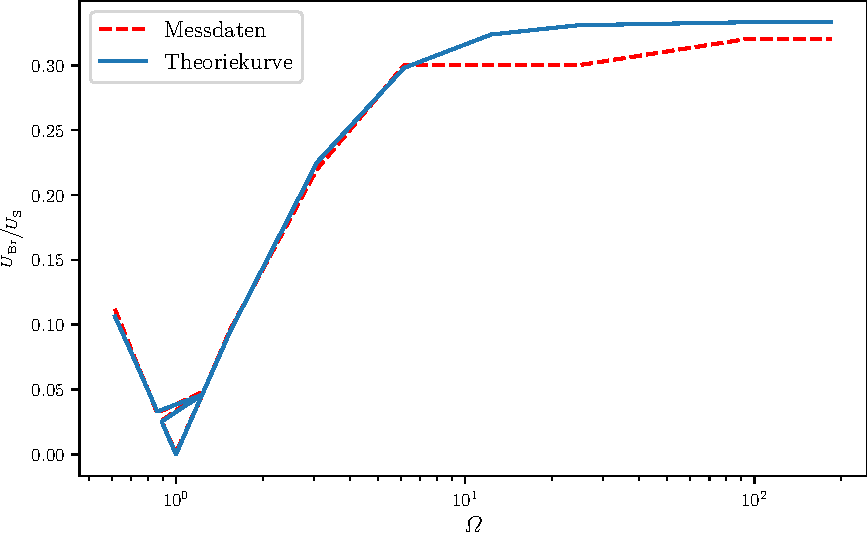
\includegraphics[width = \textwidth]{build/plot.pdf}
\end{figure}
\begin{table}
  \centering
  \caption{Gemessene Brückenspannung in Abhängigkeit von der Frequenz}
   \begin{tabular}{S[table-format = 3.2] S[table-format = 4.0]}
    \toprule
    {$v \mathbin{/} \si{\hertz} $} & {$U_\text{Br} \mathbin{/} \si{\milli\volt}$} \\
    \midrule
    100     & 340\\
    120     & 560\\
    130     & 250\\
    140     & 160\\
    200     & 240\\
    145     & 130\\
    150     & 90\\
    155     & 56\\
    160     & 20\\
    162     & 11\\
    162.56  & 9\\
    164     & 16\\
    166     & 28\\
    170     & 56\\
    175     & 80\\
    180     & 120\\
    190     & 170\\
    250     & 480\\
    500     & 1100\\
    1000    & 1500\\
    2000    & 1500\\
    4000    & 1500\\
    15000   & 1600\\
    30000   & 1600\\
    \bottomrule
   \end{tabular}
 \end{table}
 \newpage
\subsection{Klirrfaktor-Messung}
Zur Bestimmung des Klirrfaktors wird die Summe der Oberwellen (größer als 1) auf die zweite Oberwelle beschränkt.
Mit $f(2)\approx 0.149$ und $U_\text{Br}(2v_0)=\SI{0.8}{\volt}$ folgt für die Spannung der zweiten Oberwelle $U_2=\SI{5.37}{\volt}$.
Hinzu kommt der Wert $U_1=\SI{0.009}{\volt}$, welcher für die Grundwelle gemessen wurde.
Dann lässt sich der Klirrfaktor mit Formel \eqref{eqn:klirreasy} zu $k=596.57$ berechnen.
